\section{LGAD検出器}
Low-Gain-Avalanche-Diode(LGAD)検出器は、高い時間分解能が実現できる半導体検出器として期待されている。
LGAD検出器を 図\ref{fg:LGAD} に示す。詳しい構造については、第2章で解説を行う。
LGAD検出器は増幅層によって意図的に高電場を作り出すことで、電子正孔対が増幅され、立ち上がりが速く、増幅された信号を出すことができる。
電圧を上げることで、増幅層内で生じる電子雪崩による増幅率を大きくすることができる。そのため、高い時間分解能を実現することができる。
実際に、MIP粒子の測定において、30 psの時間分解能\cite{Yang_2020}を実現している半導体検出器である。

\begin{figure}[h]
    \centering
    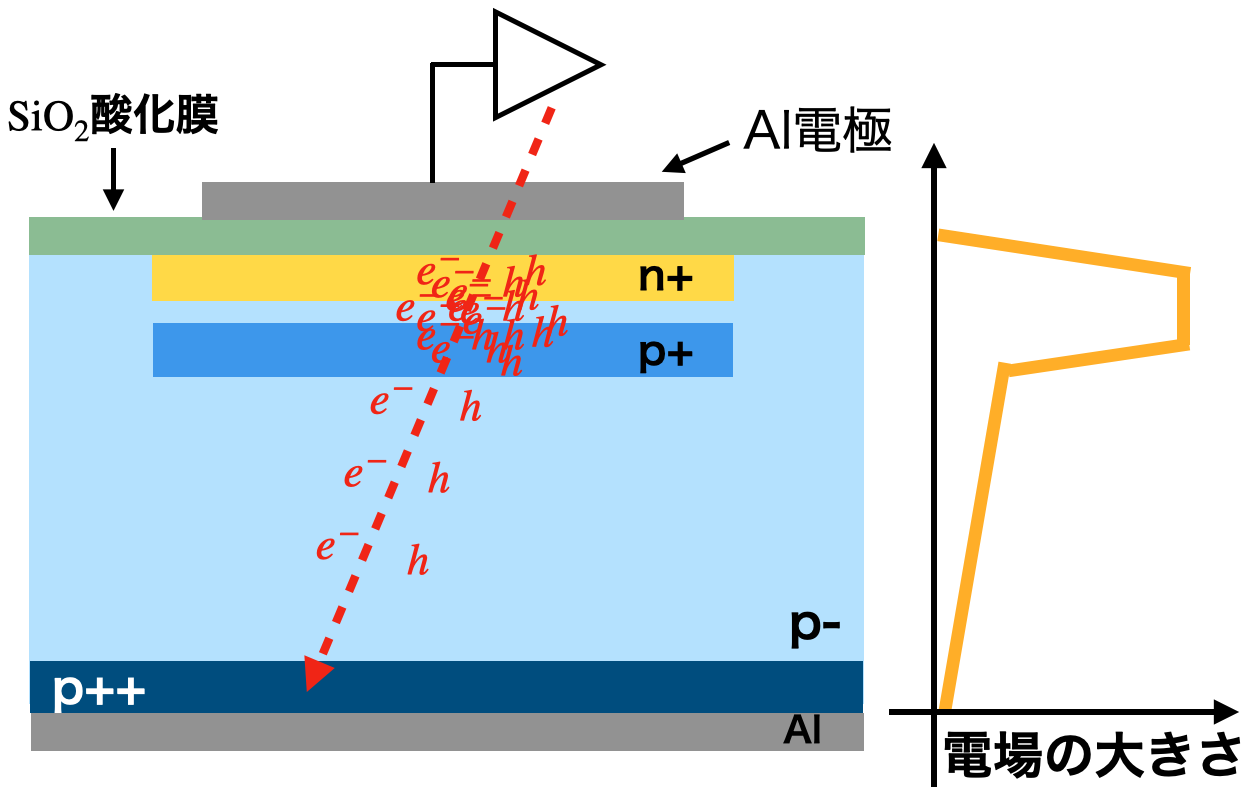
\includegraphics[width=10cm]{fig/ch1/LGAD.png}
    \caption[LGAD検出器の構造]{LGAD検出器の構造\\増幅層によって意図的に高電場を作り出し、電子雪崩によって電子正孔対が増幅される。立ち上がりの速い増幅された信号が出せるため、高い時間分解能が実現できる。}
    \label{fg:LGAD}
\end{figure}

LGAD検出器は増幅層により信号を増幅することができるため、通常の半導体検出器と比較して、
Application-Specific-Integrated-Circuit(ASIC)内のアンプの増幅率を小さく設定することができる。
そのため、アンプの増幅率の減少による消費電力の削減、そして、ASICの発熱を抑えるための冷却システムの軽減ができると考えられている。

LGAD検出器の時間分解能は以下の 式\ref{eq_TimingResolution} で表すことができるとされている。
時間分解能を構成するそれぞれの要素は、タイムウォーク$\sigma_{tw}$、ジッター$\sigma_{j}$、ランダウノイズ$\sigma_{L}$と呼ばれており、詳しい解説は第2章の第4節で行う。

\begin{equation}
    {\sigma_t}^2 = {\sigma_{tw}}^2 + {\sigma_j}^2 + {\sigma_L}^2
    \label{eq_TimingResolution}
\end{equation}

先行研究\cite{Kita_Master}から、タイムウォーク$\sigma_{tw}$、ランダウノイズ$\sigma_{L}$の影響が少ない赤外線パルスレーザーを使った測定では、
時間分解能が以下の 図\ref{fg:Kita_JittervsVoltage} のようになる。横軸が印加電圧で縦軸が時間分解能である。
赤点が$50 \rm{\mu m}$厚のStrip型、緑点が$20 \rm{\mu m}$厚のStrip型、青点が$50 \rm{\mu m}$厚のPad型、橙色の点が$20 \rm{\mu m}$厚のPad型センサーである。
$50 \rm{\mu m}$厚のPad 型センサーは、電圧が180 V付近で時間分解能が最も良く、その前後の電圧で10 V程度の時間分解能の変化がほとんどない領域が存在する。
さらに電圧を印加すると、時間分解能が悪くなることがこの研究からわかっている。

そのため、本研究ではAC-LGAD 検出器の ASIC の開発に向けた基礎特性の理解として、最も良い時間分解能を実現する増幅率を決定することと、
今後のAC-LGAD検出器の時間分解能の向上をはかるために、特に増幅率が高い場合に時間分解能が悪化する原因について理解することを目的とする。

%レーザー測定から求めた時間分解能と 式\ref{eq_Jitter} から求めたジッターを比較することで、
%\begin{equation}
%    \sigma_j = \frac{\sigma_n}{|\frac{dV}{dt}|} = \frac{\sigma_n}{\left|\frac{S}{t_r}\right|} = \frac{t_r}{\left|\frac{S}{\sigma_n}\right|}
%    \label{eq_Jitter}
%\end{equation}

%ジッター$\sigma_{j}$は以下の 式\ref{eq_Jitter} のように表すことができ、時間分解能が大きくなった原因が、
%熱ノイズの電子雪崩による影響で$\sigma_{n}$が増加したためであるとされている。

\begin{figure}[H]
    \centering
    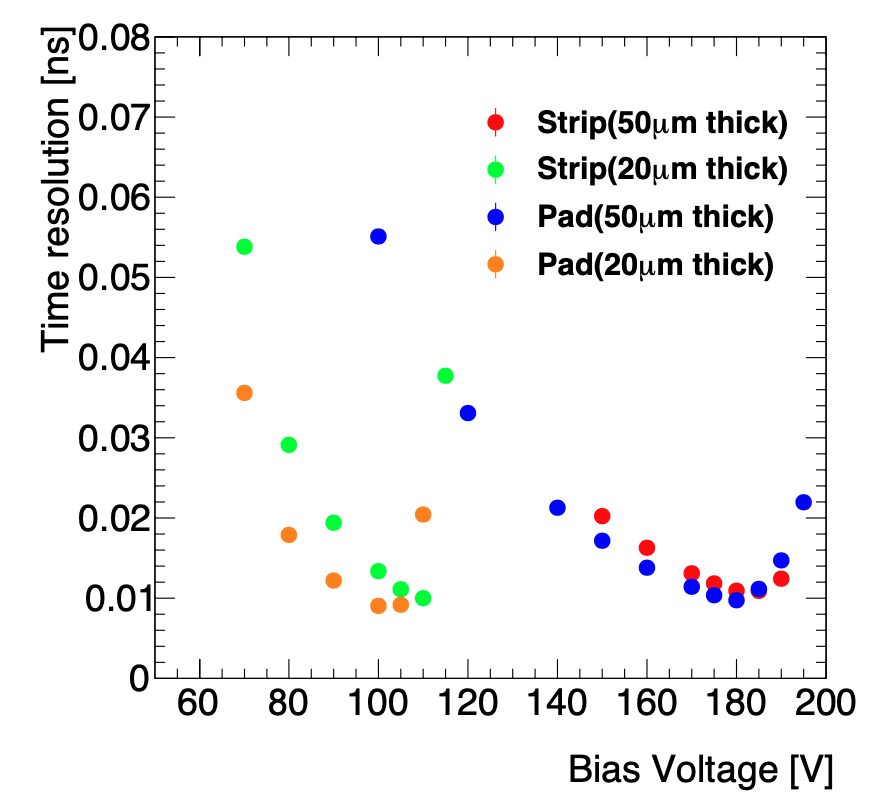
\includegraphics[width=8cm]{fig/ch1/Kita_JittervsVoltage.png}
    \caption[レーザーで測定した時間分解能(ジッター)\cite{Kita_Master}]{レーザーで測定した時間分解能(ジッター)\cite{Kita_Master}\\横軸が印加電圧で縦軸が時間分解能である。\\赤点が$50 \rm{\mu m}$厚のStrip型、緑点が$20 \rm{\mu m}$厚のStrip型、青点が$50 \rm{\mu m}$厚のPad型、橙色の点が$20 \rm{\mu m}$厚のPad型センサーである。
    $50 \rm{\mu m}$厚のPad 型センサーを示している。}
    \label{fg:Kita_JittervsVoltage}
\end{figure}




%また、LGAD検出器の信号の立ち上がり時間$t_r$、信号の大きさ$S$、ノイズ$\sigma_{n}$の測定を行い、
%式\ref{eq_Jitter} からジッターを求めることで時間分解能の詳細な構成要素について調べる。
%また、運転電圧を超える電圧で、時間分解能が増加する原因や電圧変化による時間分解能の振る舞いについて議論する。

